\documentclass[tikz,border=6pt]{standalone}
\usepackage{tikz}
\usepackage{amsmath,bm}
\usetikzlibrary{shapes.geometric, arrows.meta, positioning, fit,
                backgrounds, calc, decorations.pathreplacing}

\definecolor{graphnode}{RGB}{31,119,180}
\definecolor{csrcell}{RGB}{230,136,28}
\definecolor{highlightcell}{RGB}{214,39,40}
\definecolor{accentblue}{RGB}{70,130,180}

\begin{document}
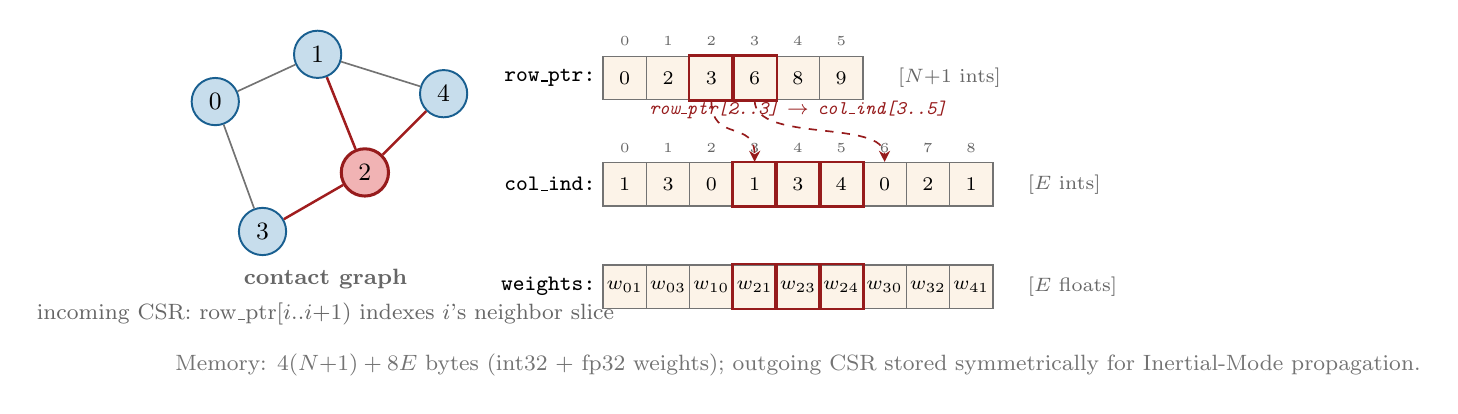
\begin{tikzpicture}[
    gnode/.style={circle, draw=graphnode!80!black, line width=0.7pt,
                  fill=graphnode!25, minimum size=0.6cm, font=\small,
                  inner sep=0pt},
    gedge/.style={-, line width=0.6pt, color=black!55},
    cell/.style={rectangle, draw=black!55, line width=0.5pt,
                 minimum width=0.55cm, minimum height=0.55cm,
                 font=\scriptsize, inner sep=1pt, fill=csrcell!10},
    hicell/.style={cell, fill=highlightcell!22, draw=highlightcell!70!black,
                   line width=0.7pt},
    arraylabel/.style={font=\footnotesize\ttfamily},
    indexlabel/.style={font=\tiny, color=black!60},
    pointer/.style={-{Stealth[length=4pt,width=4pt]}, line width=0.6pt,
                    color=accentblue!70!black, dashed},
    caption/.style={font=\footnotesize, align=center},
]

% ======================================================
% Left: 5-node contact graph.
% Node 2 is highlighted as the "focus" node whose row
% we trace through the CSR data structure.
% ======================================================
\begin{scope}[shift={(0,0)}]
  \node[gnode] (n0) at (0.00,  0.90) {0};
  \node[gnode] (n1) at (1.30,  1.50) {1};
  \node[gnode, fill=highlightcell!35, draw=highlightcell!70!black, line width=1.1pt]
        (n2) at (1.90,  0.00) {2};
  \node[gnode] (n3) at (0.60, -0.75) {3};
  \node[gnode] (n4) at (2.90,  1.00) {4};

  % undirected edges
  \draw[gedge] (n0) -- (n1);
  \draw[gedge] (n0) -- (n3);
  \draw[gedge, color=highlightcell!75!black, line width=0.9pt] (n2) -- (n1);
  \draw[gedge, color=highlightcell!75!black, line width=0.9pt] (n2) -- (n3);
  \draw[gedge, color=highlightcell!75!black, line width=0.9pt] (n2) -- (n4);
  \draw[gedge] (n1) -- (n4);

  \node[font=\footnotesize\bfseries, text=black!60] at (1.4, -1.35)
       {contact graph};
\end{scope}

% ======================================================
% Middle: CSR arrays (row\_ptr, col\_ind, weights) for the
% graph at left, drawn as aligned cells with indices above.
% ======================================================
\begin{scope}[shift={(5.2,1.20)}]
  % row_ptr: N+1 entries pointing into col_ind
  \node[arraylabel, anchor=east] at (-0.25, 0) {\texttt{row\_ptr}:};
  \foreach \v [count=\i from 0] in {0,2,3,6,8,9} {
      \node[cell] (rp\i) at (\i*0.55, 0) {\v};
      \node[indexlabel, above=0pt of rp\i] {\i};
  }
  % highlight the slice for node 2: row_ptr[2]=3 and row_ptr[3]=6
  \draw[hicell, draw=highlightcell!70!black, line width=0.9pt, fill=none]
       (rp2.south west) rectangle (rp2.north east);
  \draw[hicell, draw=highlightcell!70!black, line width=0.9pt, fill=none]
       (rp3.south west) rectangle (rp3.north east);

  \node[font=\scriptsize, text=black!60, anchor=west]
       at (6*0.55, 0) {\,[$N{+}1$ ints]};
\end{scope}

% col_ind
\begin{scope}[shift={(5.2,-0.15)}]
  \node[arraylabel, anchor=east] at (-0.25, 0) {\texttt{col\_ind}:};
  \foreach \v [count=\i from 0] in {1,3, 0, 1,3,4, 0,2, 1} {
      \node[cell] (ci\i) at (\i*0.55, 0) {\v};
      \node[indexlabel, above=0pt of ci\i] {\i};
  }
  % highlight the three neighbors of node 2: indices 3..5 ->  1, 3, 4
  \foreach \i in {3,4,5} {
      \draw[hicell, draw=highlightcell!70!black, line width=0.9pt, fill=none]
           (ci\i.south west) rectangle (ci\i.north east);
  }
  \node[font=\scriptsize, text=black!60, anchor=west]
       at (9*0.55, 0) {\,[$E$ ints]};
\end{scope}

% weights
\begin{scope}[shift={(5.2,-1.45)}]
  \node[arraylabel, anchor=east] at (-0.25, 0) {\texttt{weights}:};
  \foreach \v/\i in
    {$w_{01}$/0, $w_{03}$/1, $w_{10}$/2,
     $w_{21}$/3, $w_{23}$/4, $w_{24}$/5,
     $w_{30}$/6, $w_{32}$/7, $w_{41}$/8} {
      \node[cell] (w\i) at (\i*0.55, 0) {\v};
  }
  \foreach \i in {3,4,5} {
      \draw[hicell, draw=highlightcell!70!black, line width=0.9pt, fill=none]
           (w\i.south west) rectangle (w\i.north east);
  }
  \node[font=\scriptsize, text=black!60, anchor=west]
       at (9*0.55, 0) {\,[$E$ floats]};
\end{scope}

% ======================================================
% Pointer arrows: row_ptr[2] = 3 -> col_ind[3..5] delimits
% the neighbor slice for node 2.
% ======================================================
\draw[pointer, color=highlightcell!70!black]
     (rp2.south) .. controls ++(0,-0.55) and ++(0,0.55) .. (ci3.north);
\draw[pointer, color=highlightcell!70!black]
     (rp3.south) .. controls ++(0,-0.55) and ++(0,0.55) .. (ci6.north);

\node[font=\scriptsize\itshape, text=highlightcell!70!black]
     at (5.2 + 4*0.55, 0.80)
     {\texttt{row\_ptr[2..3]} $\to$ \texttt{col\_ind[3..5]}};

% Explanatory callout under the graph
\node[caption, text=black!60] at (1.4, -1.80)
     {incoming CSR: $\mathrm{row\_ptr}[i..i{+}1)$ indexes $i$'s neighbor slice};

% Footer note
\node[caption, text=black!55] at (5.2 + 4*0.55, -2.45)
     {Memory: $4(N{+}1) + 8E$ bytes (int32 $+$ fp32 weights);
      outgoing CSR stored symmetrically for Inertial-Mode propagation.};

\end{tikzpicture}
\end{document}
